\vspace{-1em}
\section{Framework Overview}\label{sec-arch}
We first define notation, terminology, and the problem setting that we address in this work.
Then, we formalize the two main problems that \svc addresses: (1) materialized view maintenance as data cleaning and optimizing this data cleaning, and (2) query processing on stale MVs with a sample of up-to-date data.
Finally, we overview the system architecture and discuss a numerical example of how this works in practice.

\subsection{Notation}\label{notation}
%\reminder{You have defined $\mathcal{D}$, $\{R_i\}$, etc in Definition 1. Maybe you can move Def 1 to this Section?}
\noindent \textbf{Materialized View:} Let $\mathcal{D}$ be a database which is a collection of relations $\{R_i\}$. A \emph{materialized view} $S$ is the result of applying a \emph{view definition} to $\mathcal{D}$. 
View definitions are composed of the following relational expressions:
\begin{itemize}[noitemsep] \sloppy
	\item $\sigma_{\phi}(R)$: Selection selects all tuples $r$ from $R$ that satisfy the restriction $\phi (r)$.
	\item $\Pi_{a_1,a_2,...,a_k}(R)$: Generalized projection selects attributes $\{a_1,a_2,...,a_k\}$ from $R$, allowing for new columns that are arithmetic transformations of attributes (e.g., $a_1+a_2$).
	\item $\bowtie_{\phi (r1,r2)}(R_1,R_2)$: Join selects all tuples in $R_1 \times R_2$ that satisfy $\phi (r_1,r_2)$. We use $\bowtie$ to denote all types of joins even extended outer joins such as $\rightouterjoin,\leftouterjoin,\fullouterjoin$.
	\item $\gamma_{f,A}(R)$: Apply the aggregate function $f$ to the relation R grouped by the distinct values of $A$, where $A$ is a subset of the attributes. %The result of this operation is a row with the following schema $a \in A, f_a \in f(R)$ where $a$ is the group by key and $f_a$ is the aggregate of all rows with that key.  
	The DISTINCT operation can be considered as a special case of the Aggregation operation. 
	%\footnote{A special case of this operator is $\delta$ the deduplication operator i.e. $f$ always returns null. Another special case, is when there is a expression in the group by clause which we treat as creating a set of virtual columns.}
	\item $R_1 \cup R_2$: Set union takes a union of the two sets.
	\item $R_1 \cap R_2$: Set intersection takes an intersection of the set.
	\item $R_1 - R_2$: Set difference.
\end{itemize}
The composition of relational expressions can be represented as a tree, which is called the \emph{expression tree}.
At the leaves of the tree are all of the \emph{base relations} for a view.
Each node of the tree is the result of applying one of the above relational expressions to a relation.

\vspace{.25em}

\noindent \textbf{Staleness: } We denote the set of insertions to a relation $R_i$ as $\Delta R_i$ and deletions as $\nabla R_i$.
An ``update'' to a relation can be modeled as a deletion and then an insertion.
A view $S$ is considered \emph{stale} when there exist insertions and deletions to its base relations.

\vspace{.25em}

\noindent \textbf{Maintenance: } There may be multiple ways (e.g., incremental maintenance or recomputation) to maintain a view $S$, and we denote the up-to-date view as $S'$.
We formalize the procedure to maintain the view as a \emph{maintenance strategy} $\mathcal{M}$.
A maintenance strategy is a relational expression the execution of which will update the view $S$ to produce $S'$.
It is a function of the database $\mathcal{D}$, the stale view $S$, and all the insertion and deletion relations $\{\Delta R_i\} \cup \{\nabla R_i\}$. 
In this work, we consider maintenance strategies composed of the same relational expressions as materialized views described above.
%$\mathcal{M}$ defines our data cleaning operation on the full data as it ``cleans" a stale view $S$.

%$\mathcal{M}$ is formalism that can represent incremental update, recomputation, or a mix (where some sub-expressions are recomputed and some are incrementally maintained). 

%\begin{definition}[Maintenance Strategy]\sloppy
%Let, $S$ be a materialized view.
%Formally, for a view $S$, a maintenance strategy $\mathcal{M}$ is a relational expression which is a function of the database $\mathcal{D}$, the stale view $S$, and all the insertion and deletion relations $\{\Delta R_i\} \cup \{\nabla R_i\}$.
%\end{definition}

\vspace{.25em}

\noindent \textbf{Example: }
To make the formalization of a maintenance strategy concrete, we show an example MV in Figure \ref{exexpr} based on our running example dataset.
Our example view joins the Log table with the Video table and counts the visits for each video grouped by \textsf{videoId}.
If new records have been added to \tbl{Log}, then the expressions are needed to update the view (Figure \ref{exexpr}):

\vspace{-.45em}
\begin{enumerate}[noitemsep]
\item Create a ``delta view'' by applying the view definition to \tbl{LogIns}. That is, calculate the count per video on the new logs.
\item Take the full outer join (equality on \textsf{videoId}) of the ``delta view'' and the stale view.
\item Apply the generalized projection operator to increment \textsf{visitCount} (adding the delta view \textsf{visitCount}  and the stale \textsf{visitCount} where NULL is treated as zero).
\end{enumerate}
\vspace{-.5em}

\begin{figure}[t] \vspace{-2em}
\centering
 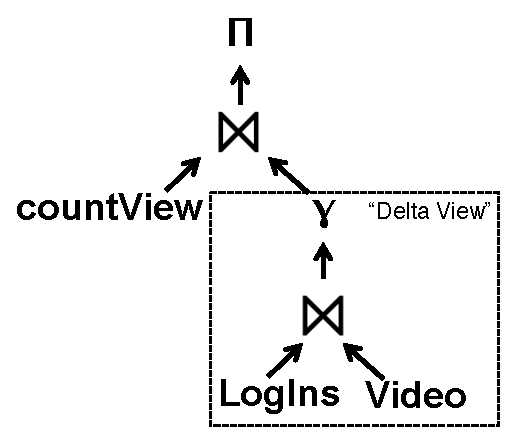
\includegraphics[scale=0.32]{figs/example_expression_tree.pdf} \vspace{-.5em}
 \caption{For our example, we represent the expression tree of the maintenance strategy. We first calculate a delta view using the new insertions and then join this view with the old view.\label{exexpr}}\vspace{-1.5em}
\end{figure}

\subsection{Sampling}
In this work, we focus on uniform samples of the rows in MVs.
We define a sampling ratio $m\in [0,1]$ and for each row in a view $S$, we include it into a sample with probability $m$.
We use the ``hat'' notation (e.g., $\hat{S}$) to denote sampled relations. 

While, uniform sampling supports a wide variety of query types, it may have issues with queries with highly selective predicates.
Stratfied sampling has been proposed to mitigate this problem as in the BlinkDB project \cite{AgarwalMPMMS13}.
However, this requires that we know our query workload in advance.  
In this paper, we do not discuss stratified sampling and will explore this further in future work.

\iffalse
Note, that this definition is slightly different from the reservoir sampling techniques studied in AQP \cite{DBLP:journals/toms/Vitter85} which find a uniform sample of fixed \emph{size} $k\le \mid S \mid$.
Our sampling ratio gives a sample of the size $k$ in expectation, however, the actual size from any given instance may be slightly different.
For large sample sizes, there is little difference between the techniques since the actual size of using a sample ratio will be close to $k$.
The uniform sample model represents our algorithm which uses hashing better and also makes the presentation of our analysis more clear.

Furthermore, any ``black-box'' uniform sampling algorithm can be used to achieve a reservoir sample.
The use of one technique over another does not affect the general principles or the statistics of \svc, only the 
notation in the analysis.
\fi

%\vspace{2em}
\subsection{Problem Statements}
\subsubsection{View Maintenance as Data Cleaning}\label{cleaning}
%In \svc, we model staleness in an MV as a type of data error.
We formalize the problem of correcting staleness as a data cleaning operation so we can apply our data cleaning approach.
In the unsampled case, $\mathcal{M}$ defines a data cleaning operation.
If we are given a materialized view $S$ and we know the base relations have had insertions and deletions, then there are three possible types of error:
(1) a row in $S$ needs to be updated, (2) a row in $S$ needs to be deleted, and (3) new row needs to be inserted into $S$.
Applying $\mathcal{M}$ removes these errors making the view ``clean".
%In the absence of these errors, we call a view \emph{up-to-date}.

However, now suppose we have a sampled view $\hat{S}$, simply applying updates to the rows in the sample may not suffice.
If new rows need to be inserted into $S$, those will never be represented in the sample violating our uniform sampling.
Thus, we define cleaning in the following way: suppose we have a stale uniform sample $\hat{S}$, cleaning this sample
should give us $\hat{S'}$ a uniform sample of the up-to-date view $S'$ with the same sampling ratio.
Formally, this can be represented as the following operations: (1) if an update is needed, update the row, (2) if a row needs to be deleted, delete the row, and (3) for all new rows that need to be inserted into the view $S$ insert a random sample of ratio $m$.

Due to the insertions, the defined data cleaning on a sample does not necessarily give a unique $\hat{S'}$, so the next question is how to formalize the link between $\hat{S}$ and $\hat{S'}$. 
To link a corresponding stale sample (dirty data) and up-to-date sample (clean data), we define the following property:
\begin{definition}[Correspondence]
$\hat{S'}$ and $\hat{S}$ are uniform samples of $S'$ and $S$, respectively.  We say $\hat{S'}$ and $\hat{S}$ correspond if and only if:
\vspace{-.25em}
\begin{itemize}[noitemsep]
\item For every row $r$ in $\hat{S}$ that required a delete, $r \not\in \hat{S'}$
\item For every row $r$ in $\hat{S}$ that required an update to $r'$, $r' \in \hat{S'}$
\item For every row $r$ in $\hat{S}$  that was unchanged, $r \in \hat{S'}$
\item For every row $r$ in $S$ but not in $\hat{S}$, $r \not\in \hat{S'}$
\end{itemize}
\vspace{-.25em}
%\item For every row $r$ in $S'$ that is newly inserted, $r \not\in \hat{S}$.
%\item If a row $r$ requires an update and then a deletion. The deletion takes precedence and $r \not\in \hat{S'}$.
%\item Rows that are inserted trivially satisfy the conditions since those rows are not contained in $S$ or $\hat{S}$.
\label{correspondence}
\end{definition}
%This definition of correspondence gives us a way to get two samples from which we can take a row-by-row difference.
%There is some nuance in how to handle null values which we discuss in Section \ref{correction}.

The goal of \svc is to efficiently produce a corresponding up-to-date sample from a stale one thus cleaning the sample.
In the first component of \svc (Section \ref{sampling}), we take as input a uniform sample of a stale view $\hat{S}$, a maintenance strategy $\mathcal{M}$, and a set of updates $\{\Delta R_i\} \cup \{\nabla R_i\}$.
We return $\hat{S'}$, a clean uniform sample (a uniform sample of $S'$) that satisfies the correspondence property with $\hat{S}$.

\iffalse
\begin{example}[Correspondence]
Suppose \tbl{countView} has 4 video rows: 
\begin{lstlisting} [mathescape]
V1 (visitCount = 4), V2 (visitCount = 6), V3 (visitCount = 1), V4 (visitCount = 1)
\end{lstlisting}
We take a sample of \tbl{countView} and call it \tbl{countViewSample} that contains V1 and V2.
\tbl{LogIns} has new logs of 1 visit for V1 and 1 visit for a new video V5.
An up-to-date sample that corresponds is:
\begin{lstlisting} [mathescape]
V1 (visitCount = 4+1), V2 (visitCount = 6)
\end{lstlisting}
An up-to-date sample that does \emph{not} corresponds is: 
\begin{lstlisting} [mathescape]
V1 (visitCount = 4+1), V3 (visitCount = 1)
\end{lstlisting}
This is because V2 was unchanged and therefore should be included in the sample.
\end{example}
\fi

\subsubsection{Query Correction}
In the query correction phase, we take a query result on a stale view and use the up-to-date sample to compensate for the staleness.
Given a query $q$ which has been applied to the stale view $q(S)$ giving a stale result.
Our query correction component takes the two corresponding samples $\hat{S'}$ and $\hat{S}$, and calculates a correction to~$q(S)$.

Like similar restrictions in other sample-based systems \cite{agarwalknowing}, there are restrictions on the queries $q$ on the view that we can answer. 
In the SampleClean work, we focused on \sumfunc, \countfunc, and \avgfunc queries of the form\footnote{\scriptsize For simplity, we exclude the group by clause for all queries in the paper, as it can be modeled as part of the \textsf{Condition}.}: 
\begin{lstlisting} [mathescape,basicstyle={\scriptsize}]
SELECT $f(a)$ FROM View WHERE Condition(A);
\end{lstlisting}
In this work, we expand the scope of the query processing, and consider general non-nested aggregate queries with predicates.

We also consider correcting stale non-nested select queries of the following form with predicates:
\begin{lstlisting} [mathescape,basicstyle={\scriptsize}]
SELECT * FROM View WHERE Condition(A);
\end{lstlisting}
As with all sample estimates, the accuracy increases with sample size, thus less selective predicates lead to more accurate results.
%From these queries, we exclude the group by clause, as we model group by clauses as part of the \textsf{Condition}.

\iffalse
\subsubsection{Outlier Indexing}
The query correction in the previous subsection is derived from a sample.
Sampling is known to be sensitive to outliers, which we define as records whose values deviate significantly from the mean.
However, a challenge is that since we do not materialize the entire up-to-date view detecting which records may be outliers is challenging.
Instead, we define an outlier index on base relations of the database $\mathcal{D}$.
This index tracks records whose attributes cross some threshold $t$.
Then, for a given view $S$, this component gives a series of rules to propagate the information from the outlier index upwards.
Basically, for every row in the view that is derived from a record in the outlier index, we ensure that it is incorporated into the sample.
We use the set of outliers to return a more accurate correction result.
\fi
%We explore the conditions under which we can make this guarantee, and discuss query processing with the outlier index in Section \ref{outlier}.

\subsection{System Architecture}
We summarize the system architecture in Figure \ref{sys-arch} in our introduction.
\svc reduces the cost of view maintenance making it feasible to apply in resource-constrained settings where frequent maintenance was once impossible.
In implementation, \svc works in conjunction with existing deferred maintenance, periodic maintenance, or periodic re-calculation solutions.
We envision the scenario where materialized views are being refreshed periodically, for example nightly.
While maintaining the entire view throughout the day may be infeasible, sampling allows the database to scale the cost with the performance and resource constraints during the day.
Then, between maintenance periods, we can provide approximately up-to-date answers for some queries.

\subsection{Example Application}
Returning to our example \tbl{countView}, suppose a user wants to know how many videos have received more than 100 views.
\begin{lstlisting}[basicstyle={\scriptsize}]
SELECT COUNT(1) FROM countView 
WHERE visitCount > 100;
\end{lstlisting}
Let us suppose the initial query result is $45$.
There now have been new log records inserted into the Log table making the old result stale.
For example, if our sampling ratio is 5\%, that means for 5\% of the videos (distinct \tbl{videoId}), we update just the view counts of those videos.
%From this sample, we calculate how many new videos changed from less than 100 views to times greater than 100; let us suppose this answer is $2$.
%Since our sampling ratio is 5\%, we extrapolate that $40$ new videos throughout the view should now be included in the count.
From this sample, we can estimate a correction (e.g., $40$) of the old result.
This means that we should correct the old result by $40$ resulting in the estimate of $45+40 = 85$.
